% This is "sig-alternate.tex" V2.1 April 2013
% This file should be compiled with V2.5 of "sig-alternate.cls" May 2012
%
% This example file demonstrates the use of the 'sig-alternate.cls'
% V2.5 LaTeX2e document class file. It is for those submitting
% articles to ACM Conference Proceedings WHO DO NOT WISH TO
% STRICTLY ADHERE TO THE SIGS (PUBS-BOARD-ENDORSED) STYLE.
% The 'sig-alternate.cls' file will produce a similar-looking,
% albeit, 'tighter' paper resulting in, invariably, fewer pages.
%
% ----------------------------------------------------------------------------------------------------------------
% This .tex file (and associated .cls V2.5) produces:
%       1) The Permission Statement
%       2) The Conference (location) Info information
%       3) The Copyright Line with ACM data
%       4) NO page numbers
%
% as against the acm_proc_article-sp.cls file which
% DOES NOT produce 1) thru' 3) above.
%
% Using 'sig-alternate.cls' you have control, however, from within
% the source .tex file, over both the CopyrightYear
% (defaulted to 200X) and the ACM Copyright Data
% (defaulted to X-XXXXX-XX-X/XX/XX).
% e.g.
% \CopyrightYear{2007} will cause 2007 to appear in the copyright line.
% \crdata{0-12345-67-8/90/12} will cause 0-12345-67-8/90/12 to appear in the copyright line.
%
% ---------------------------------------------------------------------------------------------------------------
% This .tex source is an example which *does* use
% the .bib file (from which the .bbl file % is produced).
% REMEMBER HOWEVER: After having produced the .bbl file,
% and prior to final submission, you *NEED* to 'insert'
% your .bbl file into your source .tex file so as to provide
% ONE 'self-contained' source file.
%
% ================= IF YOU HAVE QUESTIONS =======================
% Questions regarding the SIGS styles, SIGS policies and
% procedures, Conferences etc. should be sent to
% Adrienne Griscti (griscti@acm.org)
%
% Technical questions _only_ to
% Gerald Murray (murray@hq.acm.org)
% ===============================================================
%
% For tracking purposes - this is V2.0 - May 2012

\documentclass{sig-alternate-05-2015}

\usepackage[backend=biber,style=numeric,sorting=nyt]{biblatex}
\addbibresource{Paper.bib}
\begin{document}

% Copyright
%\setcopyright{acmcopyright}
%\setcopyright{acmlicensed}
%\setcopyright{rightsretained}
%\setcopyright{usgov}
%\setcopyright{usgovmixed}
%\setcopyright{cagov}
%\setcopyright{cagovmixed}

% DOI
%\doi{10.475/123_4}

% ISBN
%\isbn{123-4567-24-567/08/06}

%Conference
%\conferenceinfo{PLDI '13}{June 16--19, 2013, Seattle, WA, USA}

%\acmPrice{\$15.00}

%
% --- Author Metadata here ---
%\conferenceinfo{WOODSTOCK}{'97 El Paso, Texas USA}
%\CopyrightYear{2007} % Allows default copyright year (20XX) to be over-ridden - IF NEED BE.
%\crdata{0-12345-67-8/90/01}  % Allows default copyright data (0-89791-88-6/97/05) to be over-ridden - IF NEED BE.
% --- End of Author Metadata ---

%%%%%%%%%%%%%%%%%%
%TITLE
%%%%%%%%%%%%%%%%%%
\title{Marster Gesture for Public}
%\subtitle{[Extended Abstract]



%\title{Alternate {\ttlit ACM} SIG Proceedings Paper in LaTeX
%Format\titlenote{(Produces the permission block, and
%copyright information). For use with
%SIG-ALTERNATE.CLS. Supported by ACM.}}
%\subtitle{[Extended Abstract]
%\titlenote{A full version of this paper is available as
%\textit{Author's Guide to Preparing ACM SIG Proceedings Using
%\LaTeX$2_\epsilon$\ and BibTeX} at
%\texttt{www.acm.org/eaddress.htm}}}
%
% You need the command \numberofauthors to handle the 'placement
% and alignment' of the authors beneath the title.
%
% For aesthetic reasons, we recommend 'three authors at a time'
% i.e. three 'name/affiliation blocks' be placed beneath the title.
%
% NOTE: You are NOT restricted in how many 'rows' of
% "name/affiliations" may appear. We just ask that you restrict
% the number of 'columns' to three.
%
% Because of the available 'opening page real-estate'
% we ask you to refrain from putting more than six authors
% (two rows with three columns) beneath the article title.
% More than six makes the first-page appear very cluttered indeed.
%
% Use the \alignauthor commands to handle the names
% and affiliations for an 'aesthetic maximum' of six authors.
% Add names, affiliations, addresses for
% the seventh etc. author(s) as the argument for the
% \additionalauthors command.
% These 'additional authors' will be output/set for you
% without further effort on your part as the last section in
% the body of your article BEFORE References or any Appendices.

%%%%%%%%%%%%%%%%%%
%AUTHOR LISTING
%%%%%%%%%%%%%%%%%%
\numberofauthors{5} %  in this sample file, there are a *total*
% of EIGHT authors. SIX appear on the 'first-page' (for formatting
% reasons) and the remaining two appear in the \additionalauthors section.
%
\author{
% You can go ahead and credit any number of authors here,
% e.g. one 'row of three' or two rows (consisting of one row of three
% and a second row of one, two or three).
%
% The command \alignauthor (no curly braces needed) should
% precede each author name, affiliation/snail-mail address and
% e-mail address. Additionally, tag each line of
% affiliation/address with \affaddr, and tag the
% e-mail address with \email.
%
% 1st. author
\alignauthor
Jeni Paay\titlenote{Dr.~Paay insisted her name be first. :P}\\
       \affaddr{Research Centre for Socio-Interactive Design}\\
       \affaddr{Selma Lagerlofs Vej 300}\\
       \affaddr{Aalborg East 9220, Denmark}\\
       \email{Jeni@cs.aau.dk}
% 2nd. author
\alignauthor
Bjarke Martin Lauridsen\\
       \affaddr{Institute for Computer Science}\\
       \affaddr{Selma Lagerlofs Vej 300}\\
       \affaddr{Aalborg East 9220, Denmark}\\
       \email{blauri10@student.aau.dk}
% 3rd. author
\alignauthor
Elias Ringhauge\\
       \affaddr{Institute for Computer Science}\\
       \affaddr{Selma Lagerlofs Vej 300}\\
       \affaddr{Aalborg East 9220, Denmark}\\
       \email{eringh10@student.aau.dk}
\and  % use '\and' if you need 'another row' of author names
% 4th. author
\alignauthor
Eric Vignola Ruder\\
       \affaddr{Institute for Computer Science}\\
       \affaddr{Selma Lagerlofs Vej 300}\\
       \affaddr{Aalborg East 9220, Denmark}\\
       \email{eruder10@student.aau.dk}
% 5th. author
\alignauthor
Ivan Svilenov Penchev\titlenote{This author is the
one who did all the really hard work.}\\
       \affaddr{Institute for Computer Science}\\
       \affaddr{Selma Lagerlofs Vej 300}\\
       \affaddr{Aalborg East 9220, Denmark}\\
       \email{ipench14@student.aau.dk}
}
% 6th. author
%\alignauthor Charles Palmer\\
%       \affaddr{Palmer Research Laboratories}\\
%       \affaddr{8600 Datapoint Drive}\\
%       \affaddr{San Antonio, Texas 78229}\\
%       \email{cpalmer@prl.com}
%}
% There's nothing stopping you putting the seventh, eighth, etc.
% author on the opening page (as the 'third row') but we ask,
% for aesthetic reasons that you place these 'additional authors'
% in the \additional authors block, viz.

%\additionalauthors{Additional authors: John Smith (The Th{\o}rv{\"a}ld Group,
%email: {\texttt{jsmith@affiliation.org}}) and Julius P.~Kumquat
%(The Kumquat Consortium, email: {\texttt{jpkumquat@consortium.net}}).}
%\date{30 July 1999}
% Just remember to make sure that the TOTAL number of authors
% is the number that will appear on the first page PLUS the
% number that will appear in the \additionalauthors section.


\maketitle %Must be after autor declaration as it also makes that part
\keywords{ACM proceedings; \LaTeX; text tagging}
%%%%%%%%%%%%
%INPUTS
%%%%%%%%%%%%
% !TEX root = ../paper.tex
\begin{abstract}
\todo[inline]{Write abstract}

\todo{Add section numbers to each section because of references to certain sections of the paper}

\end{abstract}

% !TEX root = ../literature.tex
\section{Introduction}
Weiser\cite{Weiser:1991} points out:
 
{\em``Ubiquitous computing names the third wave in computing, just now beginning. First were mainframes, each shared by lots of people. Now we are in the personal computing era, person and machine staring uneasily at each other across the desktop. Next comes ubiquitous computing, or the age of calm technology, when technology recedes into the background of our lives.''}.

Weiser's vision of ubiquitous computing, is over 20 years old, includes the ubiquity availability of computers that are preferably not distinguishable from everyday objects. He also talks about "calm technology", which is this technology that resides in the periphery and plays a non-dominant role in a user's life. The perception of devices plays a major role in Weiser's vision, however the other side of that is availability of devices and also computing power, which is important for cross-device interaction. As so we could contend and regard that the latest incarnation of Weiser's vision is cross-device interaction, where ideally joining several devices would lead to single seamless, and natural user interaction, flexible, and not restricted to a few configurations\cite{Radle:2015}.
In order for this interaction to happen we need to remain as close as possible to the real world and have multimodality in mind, as Jain et al. states: ``human interaction with the world is multi-modal, and rich multi-modal interaction is part of what defines a natural experience.''\cite{Jain:2011}. 
This corresponds well witth the way Wigdor and Wixon defines NUI , where "Natural" is about how the users feel and what they do when using a product. The products must mirror the user's capabilities and meet their needs, but the trick is to help the users feel comfortable about the product without the need for much practice\cite{Wigdor:2011}. This becomes important for the design of product that has a non-dominant role in a user's life as the user should not be using a lot of time for adapting to the products.   
Ideally we would see a combination of multiple modalities, for instance gestures, augmented reality, touch, voice recognition etc. 
Researchers have made and published breakthroughs and designers constructed innovation design in each modality individually, however there has only been little research and work in combining them \cite{Jain:2011}. \\

It is possible for the existence of untapped opportunities in the integration of multiple natural user interaction modalities for enriching the cross-device experience with hand-held devices and large public displays. \\

In this paper we review the research that has been done within interaction with large displays. 
This has been done to map the current understanding and practices, thereby helping future researchers, within this field, to gain a perspective as well as identifying possible untapped opportunities for future work.
% !TEX root = ../paper.tex
\section{MAIN}
libum larum detoritidididadadad lalalamothumsto o nagasaki witsjomudanagu omahaski \\
This is a test cite \cite{Walter:2014}, this should refference Walter 2014 %Background
% !TEX root = ../paper.tex
\section{Findings}
libum larum detoritidididadadad lalalamothumsto o nagasaki witsjomudanagu omahaski \\
This is a test cite \cite{Walter:2014}, this should refference Walter 2014 %...
% !TEX root = ../literature.tex
\subsection{Discussion}
%this section needs to be called discussion, and you need to use it to discuss a bit more about the relationships between the different fields, concluding with the idea that some sharing of information across these areas to futher research various aspects would be a good idea. So you are on the right track - but you need to be a bit more detailed in your thinking
This current paper aims to analytically summarize published research within the areas of interaction with large displays, natural user interaction, and cross device interaction.In this section we expand on the relationships between presented different fields, we believe this will further deepen our understanding of them.

%The findings of this work are that gesture recogntion using touchscreens is now a mature enough technology that it is ready for implementation in commerical products. The iPhone has shown that basic gesturing has a place in mobile operating systems and my results show that more complex gestures can be easily recognised and recognised accurately. The problem is context.
By making the objects that surround us change their non-interactive state to a responsive medium, Buxton and Welnner achieved a novelty supporting Weiser's vision of ubiquitous computing. A secondary objective of Weiser was related to the size of the object. An example of this principle can be related to the work of Czerwinski that shows how size can correlate to the performance in a work environment.

A new state is often related to not only a technologically progress but also conceptual ideas. A Technological example would be the development of the Kinect that provide new interaction possibilities\cite{Wilson:2010}, and a conceptual example is to use tangible objects as a medium for interacting with the virtual world\cite{Rekimoto:1997, Keefe:2001}.
This change provides new opportunities and challenges for developing interaction techniques in the interaction space of natural user interaction and cross-device interaction. These two identified areas differ in-between, however they also have common ground, we present this idea in \Cref{fig:litreview}.\\

We reflect upon how the shift from private to public environment correlates with the challenges in natural user interaction and cross-device interaction for interaction techniques.
While there isn't a specific formula covering the creation of an ideal interaction technique, there are some guidances. For example Brignull advices to make the transition between an onlooker to participant less socially awkward. Cheung shows that their are specific barriers for interacting and presents a diagram of each state when said challenges are encountered, he advices that those should be addressed in every case. However we notice that the majority of papers we examined do not explicitly focus on the environment, instead they present unique solutions, without beforehand taking into consideration the settings.
From the research done on public space and public display we are able to identify 3 elements that directly impacts the creation of interaction techniques: \emph{accessibility}, \emph{learn-ability}, and \emph{social acceptance}. To interact with a system it is necessary that the technique can be used without obstacles. For instance a large display can be interacted with by either touch or mid-air gestures, but mid-air gestures risks being interrupted by people who walks between the user and the sensor. It is also important that the user understands how to interact with the system and \emph{``move beyond ephemeral interactions, driven by the playfulness of the interface''}\cite{Jacucci:2010}, especially for a public walk-up-and-use system. However in the end for the user to engage in using the system, the interaction technique must be acceptable in a social circumstances to avoid intimidating or embarrassing the user. 
% The reoccurring challenges for interaction techniques in the public environment are: social acceptability, learning curve, 

With this limitation came different approaches for solving it. 
We identified two different areas which deals with it, we present them in \Cref{fig:litreview}.
\begin{figure}[h!]
\centering
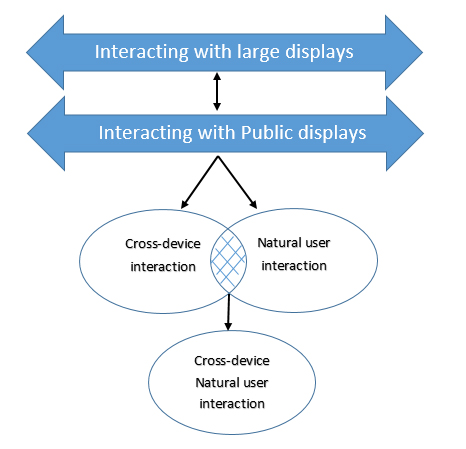
\epsfig{file=images/litreview-fig1.jpg, width=0.5\textwidth}
\caption{Write Caption}
\label{fig:litreview}
\end{figure}
%\todo[inline]{Assuming the numbers are right, then keep this. But for god sake, use cite!}
The fields of natural user interactions and cross-device interactions were examined. 
We were surprised to see that research in combining features from the two areas is slim even though they are complementary to each other. 
There was research that was done [26, 27, 28, 29]. 
Interaction-techniques were evaluated with 3-6 people using qualitative surveys in [27,28,29] and without qualitative surveys in [26].\\

In summary, we can see research opportunities in further exploration of cross-device natural user interactions technique for large displays. We believe the limitations that each of these fields ignore is the interaction space between them. To move beyond this limitation, we believe a unification of these discrete interaction techniques in continuous interaction space and it's further research would be positive and beneficial.
Firstly, as handheld devices become thinner and lighter and spatially-aware technologies, such as Kinect, continue to evolve, this opens a potentially rich space of aforementioned techniques. 
Secondly, we see opportunities in quantitative aspect, for example comparative study of different interaction techniques. 

\section{Conclusion}\label{Sec:Conclusion}
In this paper we presented an overview of HCI research within interacting with large displays. We reviewed 34 papers from the last decade in detail. A picture (\Cref{fig:litreview}) was drawn about the relation of large displays, public displays, cross-device interaction and natural user interaction. Cross device interaction and natural user interaction was found to be a subset of large- and public displays. Based on further examination of these areas in research, we identified cross-device natural user interaction as well as some opportunities and shortcomings that we used to suggest possible future research areas.\\
In the future we would like to see quantitative research within the field of cross-device natural user interaction, as well as use of the produced statistically solid results as a guide for the design of further applications for cross-device interactions and large displays.

%Refferences and apendix are just after this weird block

%%%%%%%%%%%%%%%%%%%%%%%%%%%%%%%%%%%%%%%%%%%%%%%
% CCSXML IF needed
%
% The code below should be generated by the tool at
% http://dl.acm.org/ccs.cfm
% Please copy and paste the code instead of the example below. 
%
%\begin{CCSXML}
%<ccs2012>
% <concept>
%  <concept_id>10010520.10010553.10010562</concept_id>
%  <concept_desc>Computer systems organization~Embedded systems</concept_desc>
%  <concept_significance>500</concept_significance>
% </concept>
% <concept>
%  <concept_id>10010520.10010575.10010755</concept_id>
%  <concept_desc>Computer systems organization~Redundancy</concept_desc>
%  <concept_significance>300</concept_significance>
% </concept>
% <concept>
%  <concept_id>10010520.10010553.10010554</concept_id>
%  <concept_desc>Computer systems organization~Robotics</concept_desc>
%  <concept_significance>100</concept_significance>
% </concept>
% <concept>
%  <concept_id>10003033.10003083.10003095</concept_id>
%  <concept_desc>Networks~Network reliability</concept_desc>
%  <concept_significance>100</concept_significance>
% </concept>
%</ccs2012>  
%\end{CCSXML}

%\ccsdesc[500]{Computer systems organization~Embedded systems}
%\ccsdesc[300]{Computer systems organization~Redundancy}
%\ccsdesc{Computer systems organization~Robotics}
%\ccsdesc[100]{Networks~Network reliability}
%%%%%%%%%%%%%%%%%%%%%%%%%%%%%%%%%%%%%%%%%%%%%%%

%
%  Use this command to print the description
%
%\printccsdesc  (no idea what it is used  for)


%%%%%%%%%%%%
%REFFERENCE SECTION
%%%%%%%%%%%%
\printbibliography[heading=bibnumbered, title={Refferences}]
%
% ACM needs 'a single self-contained file'!
%

%%%%%%%%%%%%%%%%%%%
%APPENDICES are optional
%\balancecolumns
\appendix % THIS SETS A STYLE
%Appendix A
\section{Headings in Appendices}
The rules about hierarchical headings discussed above for
the body of the article are different in the appendices.
In the \textbf{appendix} environment, the command
\textbf{section} is used to
indicate the start of each Appendix, with alphabetic order
designation (i.e. the first is A, the second B, etc.) and
a title (if you include one).  So, if you need
hierarchical structure
\textit{within} an Appendix, start with \textbf{subsection} as the
highest level. Here is an outline of the body of this
document in Appendix-appropriate form:
\subsection{Introduction}
\subsection{The Body of the Paper}
\subsubsection{Type Changes and  Special Characters}
\subsubsection{Math Equations}
\paragraph{Inline (In-text) Equations}
\paragraph{Display Equations}
\subsubsection{Citations}
\subsubsection{Tables}
\subsubsection{Figures}
\subsubsection{Theorem-like Constructs}
\subsubsection*{A Caveat for the \TeX\ Expert}
\subsection{Conclusions}
\subsection{Acknowledgments}
\subsection{Additional Authors}
This section is inserted by \LaTeX; you do not insert it.
You just add the names and information in the
\texttt{{\char'134}additionalauthors} command at the start
of the document.
\subsection{References}
Generated by bibtex from your ~.bib file.  Run latex,
then bibtex, then latex twice (to resolve references)
to create the ~.bbl file.  Insert that ~.bbl file into
the .tex source file and comment out
the command \texttt{{\char'134}thebibliography}.
% This next section command marks the start of
% Appendix B, and does not continue the present hierarchy
\section{More Help for the Hardy}
The sig-alternate.cls file itself is chock-full of succinct
and helpful comments.  If you consider yourself a moderately
experienced to expert user of \LaTeX, you may find reading
it useful but please remember not to change it.
%\balancecolumns % GM June 2007
% That's all folks!

\end{document}